\chapter{Experiment result}

\section{Baseline model}
%In ourThe data selection was run four time until it does in iteration number 3. 
As presented in the previous chapters, the baseline data selection works as following:
\begin{enumerate}
\item train a GMM-HMM and then TDNN acoustic model(AM) on 100 hour randomly selected training set(with closed caption)
\item recognize the training set using this acoustic model 
\item compute  phone matched error rate and average word duration
\item reject segments(utterances) which does not satisfy the AWD range($0.165 \leq AWD \leq 0.66$)
\item sort and select new data based on the lowest phone matched error rate. Retrain an acoustic model using the selected data. Repeat steps 1-5.
\end{enumerate}
To evaluate how good the data selection is, we recognize the development set and compute word error rate. If the word error rate decreases, the iteration can continue; otherwise, stop the iteration.

Figure \ref{awd} shows the average word duration of data selection iteration 0, 1, and 2. The X-axis is the value of average word duration, while the Y-axis represents the cumulative duration of audio in percentage. All utterances are sorted based on AWD to draw this figure. Two vertical line represents boundaries to select utterances. The utterances which are inside these two lines(the value of AWD is in the range $0.165 \leq AWD \leq 0.66$) will be selected. The result shows that less than 15\% data are rejected. Selection by using AWD is important to reject utterances which are badly aligned.

Figure  \ref{pmer} demonstrates the phone matched error rate of all iterations. The X-axis and Y-axis represent the value of PMER of each utterance and the duration of audio in percentage respectively. All utterances are sorted based on PMER to generate this figure. The value of PMER decreases slightly over several iterations where more and more utterances have less PMER in the next iteration. Nevertheless, the iteration stops in iteration three because the data selection converges(no further improvement in PMER).

\begin{center}
\label{tab:werper}
\captionof{table}{WER and PER of acoustic models}
\begin{tabular}{| c | c | c | c | c | c |   }
\hline
No. & Model & WER(\%) & PER(\%) & PMER thresh(\%) \\ \hline
1 &  baseline 0 & 43.9 & 35.8 & 36.0  \\ \hline
2 &  baseline decoding & 42.3 & 34.3 & 45.98 \\ \hline
3 &  baseline WMER & 41.2 & 34.1 & \\ \hline
4 &  baseline 1 & 41.2 & 33.8  & 35.71 \\ \hline
5 & baseline 2 & 40.5 & 33.3  & 35.44 \\ \hline
6 & baseline 3 & 40.5 & 33.3  &  \\ \hline
\end{tabular}
\end{center}

Table \ref{tab:werper} shows the result of the recognition experiments. The second column denotes the model name; the third and forth represents the value of WER and PER respectively of the corresponding model. The last column shows the PMER threshold. When we finish building a speech recognizer, we recognize the train.200 training set and select 100 hours data for the next iteration. The selection is thresholded by PMER threshold, shown in the last column.

\begin{itemize}
\item Baseline 0(row 1)  is the initial data selection iteration(iteration 0) where the training set is randomly 100 hours selection from 200 hours of training set. We evaluated baseline 0 which resulted in $43.9\%$ WER and $35.8\%$ PER. Then, we re-recognize train.200 and selected top 100 hours data with PMER threshold $36\%$.
\item Baseline decoding(row 2) utilizes the audio data and the decoding results(in place of the closed captions) of the previous iteration(baseline 0) as the new training set.
\end{itemize}


 Baseline WMER(row 3) and baseline 1(row 4) use the audio data and the closed captions(with new PMER and AWD) as the new training set. However, baseline WMER sorts utterances based on WMER instead of PMER. In contrast, baseline 1 utilized the same method as described in \ref{ch3:dataselection}. Consequently, using closed captions and sorting by PMER are the best; thus, the next iteration only experiments with closed captions as training set and sorting by PMER. Baseline 2 and 3 are the second and third(last) iteration respectively. They have the same value of WER; hence, the iteration stops because the data selection has converged.



\begin{figure}
\caption{Average word duration of data selection iterations}
\label{awd}
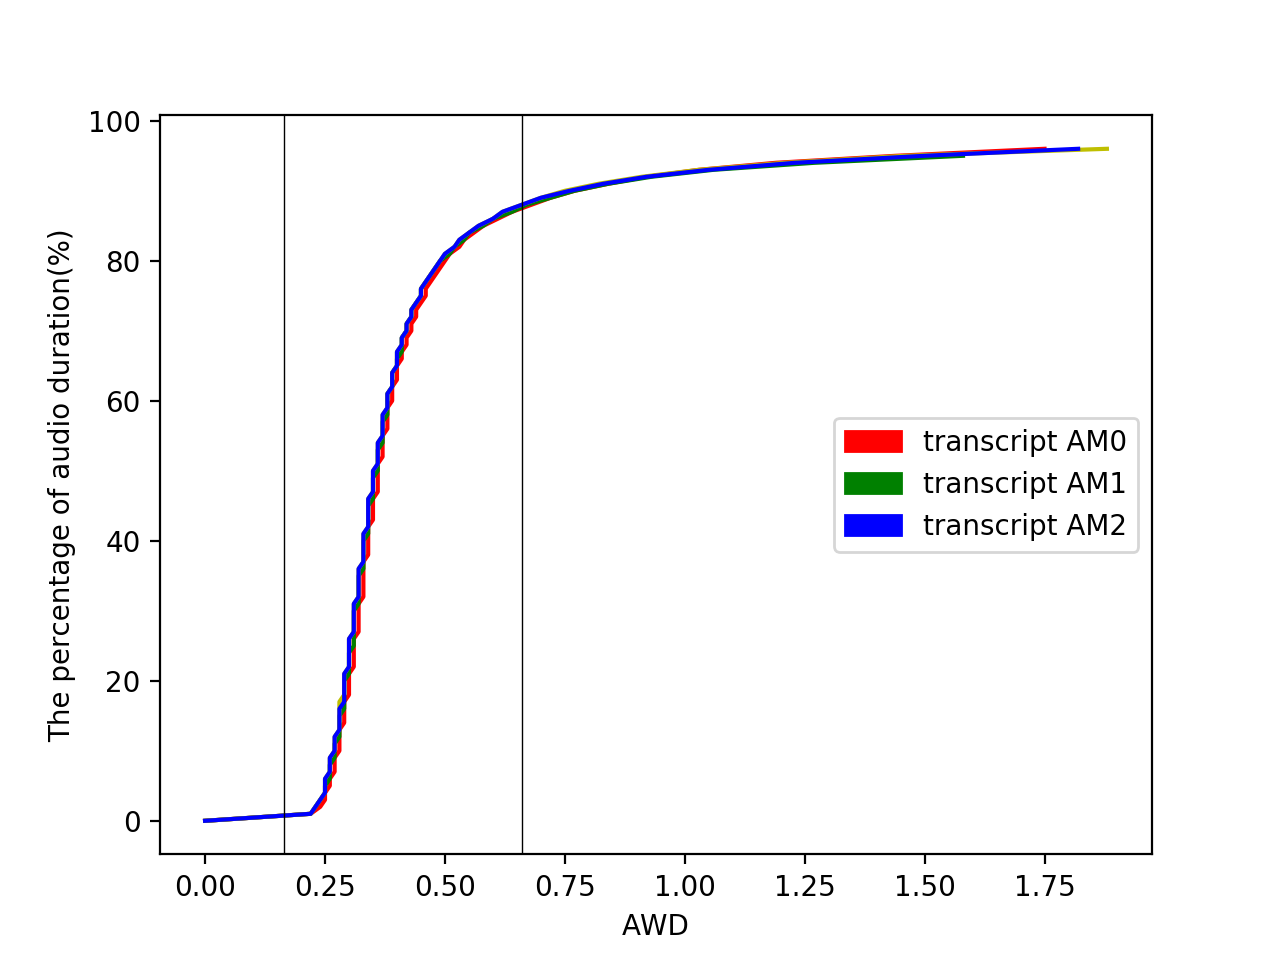
\includegraphics[scale=0.7]{awd} 
\centering
\end{figure}

\begin{figure}
\caption{Phone matched error rate of the iteration}
\label{pmer}
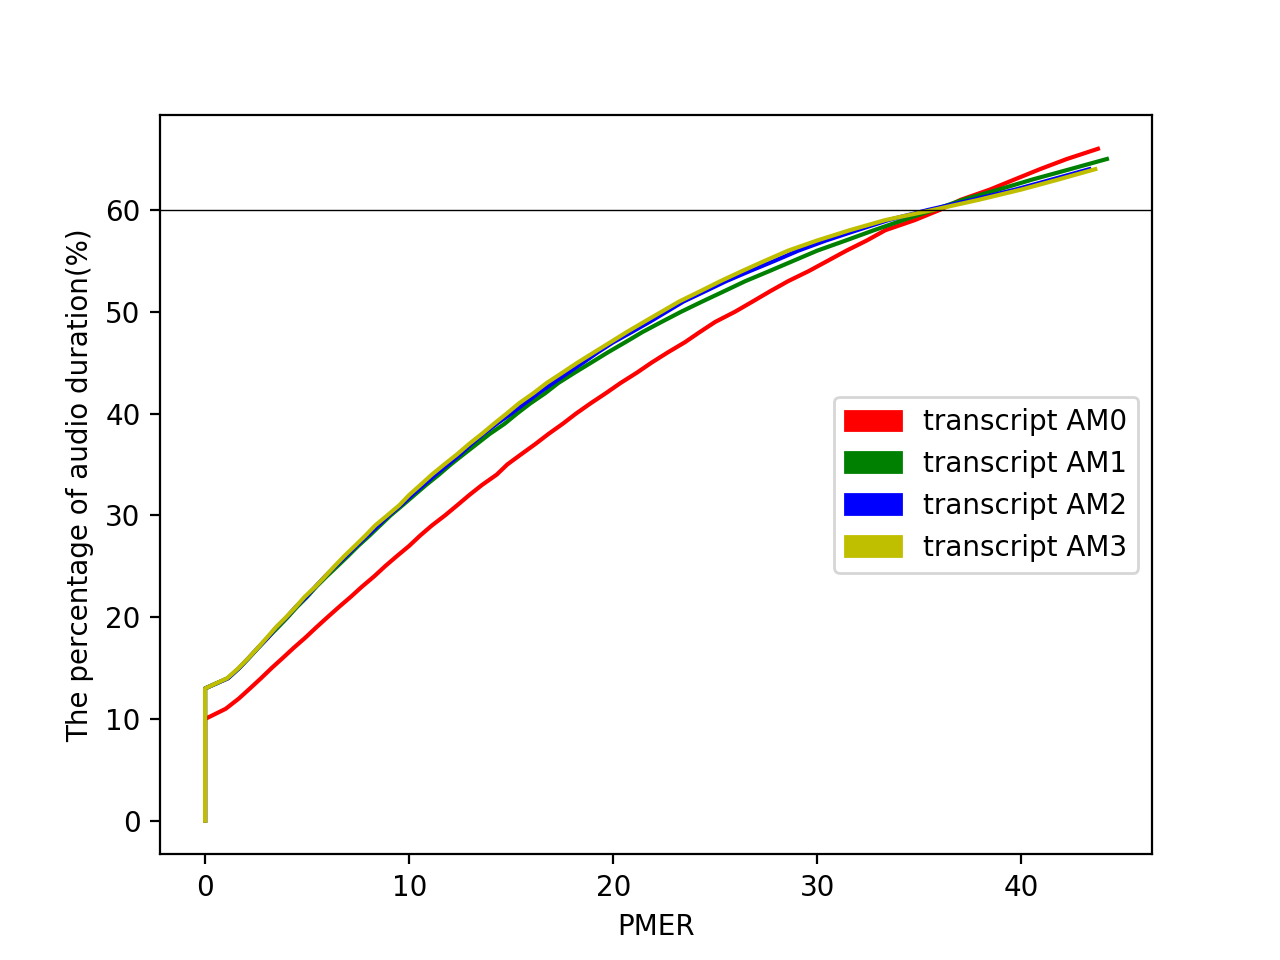
\includegraphics[scale=0.7]{pmer} 
\centering
\end{figure}




\section{Proposed models}

In addition to the baseline model, we proposed three new models which we hoped it would increase the performance. Table \ref{tab:proposedModel} demonstrates the result of our technique. Baseline 1 and 2 are the same model as shown in Table \ref{tab:werper}, while other rows show the results of the proposed models.  We put baseline 1 and 2 to compare with the proposed models.

As explained in Section \ref{proposedModels}, we proposed three new models:
\begin{enumerate}
\item Average PMER and AWD of three ASRs.  \\
By using the baseline acoustic model in baseline 1, three different ASRs were created by varying three different language models(as mentioned in \ref{3LM}). Each ASR from the three ASRs recognized the full training set and calculated new PMER and AWD. Each corresponding segment in three ASRs averages their PMER and AWD. The averaged training set is selected with the data selection method and trained to generate a new acoustic model. The new acoustic model with LM.7weeks+sub and the lexicon is evaluated as shown in model proposed average(row 3). Because the model does not improve the performance as good as baseline 2, we do not continue to the next iteration.

\item Combine three ASRs.  \\
We combined the recognition of three ASRs from Baseline 1 by using the algorithm explained in Listing \ref{algoCombine}, and then, we train a new acoustic model from the data. We evaluated the performance of the new model as shown in row 4. The value of WER of row 4(proposed combination 1) and WER of row 2(baseline 2) are the same; but, the PER decreases by 0.1. Therefore, we continue the iteration to see if it can further reduce the error rate.

Then, three ASRs of proposed combination 1 were combined and trained a new acoustic model based on the combination algorithm(Listing \ref{algoCombine}). We evaluated the new model and showed the result in row 5. Unfortunately, the performance of the model becomes poorer. The reason behind this is the combination algorithm tries to fix the bad closed captions by replacing with the decoding transcriptions if two ASRs agree(has exactly the same decoding results).

\item Utilize a randomly different random training set.  \\
We select a different full training set, and then, we used the baseline model 2 to recognize the new training set. The closed captions of the new training set and their corresponding PMER and AWD are used for training a new acoustic model. The new model is evaluated and written in row 6. It shows better performance by reducing WER as well as PER by 0.1. Again, we do another iteration, select a new training set randomly, and evaluate the new model(row 7). Unfortunately, the performance becomes worse compared to baseline 2. There is a luck factor in this technique. If we choose a very good training set in the next iteration, we may obtain a better performance model. Otherwise, the error rate can get worse as shown in row 7.

\end{enumerate} 

%\begin{figure}[H]
%\caption{Average phone duration}
%\label{apd}
%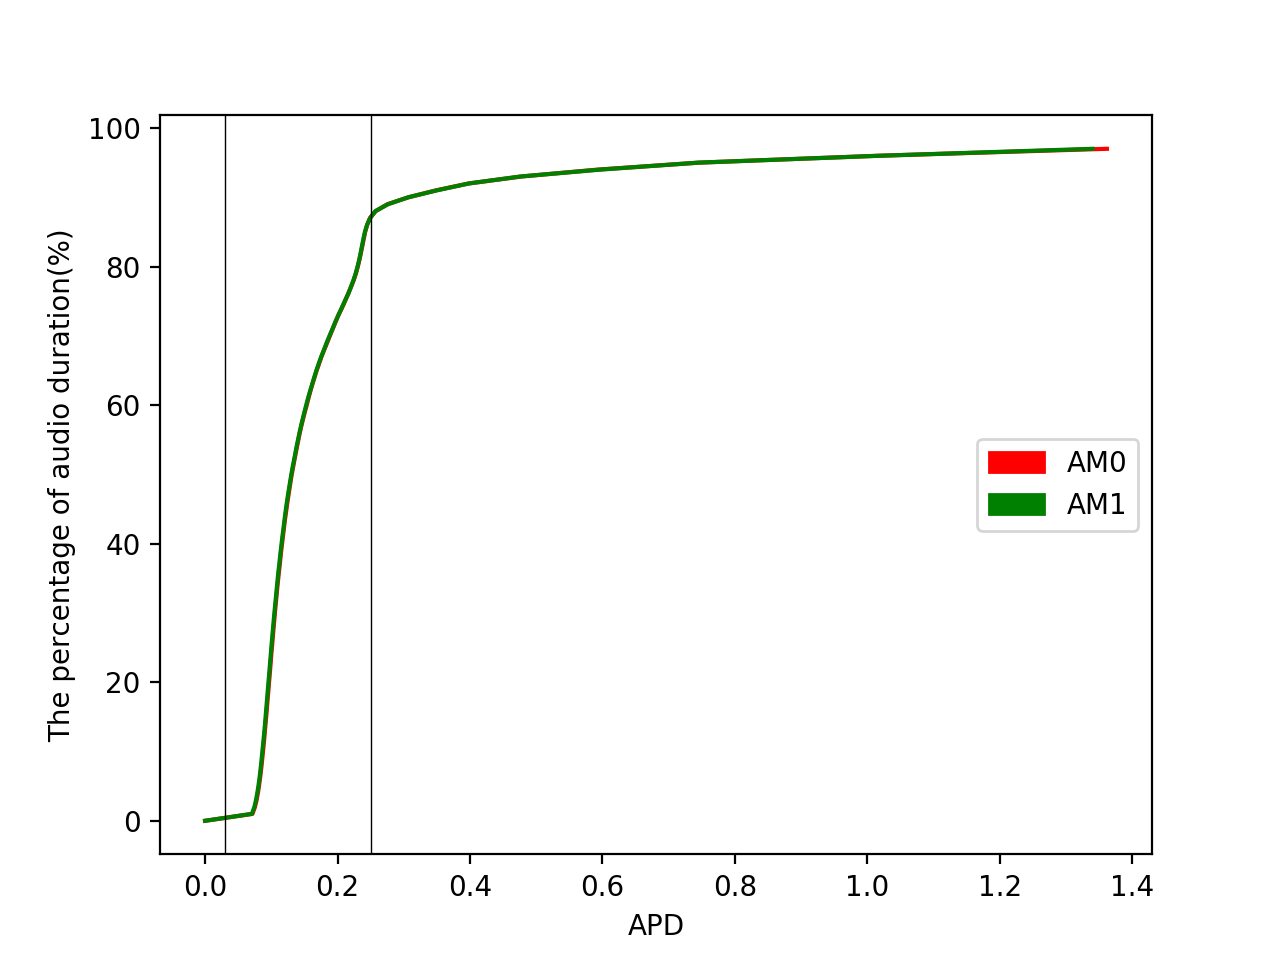
\includegraphics[scale=0.7]{apd} 
%\centering
%\end{figure}

% proposed combination 1 from 
% proposed combination 2
%different data set 1 from baseline 2
%different data set 2 from different data set 1

\begin{center}
\label{tab:proposedModel}
\captionof{table}{WER and PER of baseline versus proposed model}
\begin{tabular}{ | c | c | c | c | c |   }
\hline
No.  & model name & WER(\%) & PER(\%) \\ \hline
1  & baseline 1 & 41.2 & 33.8  \\ \hline
2  & baseline 2 & 40.5 & 33.3  \\ \hline
3 & proposed average & 41 & 33.7 \\ \hline
4 & proposed combination 1 & 40.5 & 33.2 \\ \hline
5 & proposed combination 2 &  41.6 & 33.7  \\ \hline
6 & different data set 1 & 40.4 & 33.2 \\ \hline
7 & different data set 2 & 40.7 & 33.6 \\ \hline
\end{tabular}
\end{center}

\section{Execution time}

Table \ref{tab:exectime} shows the execution time of each data selection iteration. The most demanding process is to train an acoustic model. The second most demanding process is to recognize the full training set and select  a good subset of data from it. This is time consuming due to a massive volume of training data(around 200 hours of TV broadcasts). In overall, the execution time of each iteration roughly takes 43 hours. 

\begin{center}
\label{tab:exectime}
\captionof{table}{WER and PER of baseline versus proposed model}
\begin{tabular}{ | c | c | c | c | c | c | c |   }
\hline
Itera & Train & Recognize \&  & Calculate & Decoding graph  & Decoding graph  & Total \\ 
-tion & AM &  data selection & WER & with LM.200 &  with LM.7weeks+subs & \\ \hline
0 & 21h & 16h & 1h & 6m & 5h & 43h  \\ \hline
1 & 24h & 14h & 1h & 5m & 3h & 43h  \\ \hline
\end{tabular}
\end{center}

\section{Discussion}
This chapter provides the results of experiments of baseline and proposed approaches. In this section, we give a summary of our experiments and offer possible explanations for the obtained results.

In baseline model, we showed a chart of PMER(see \ref{pmer}) produced by four iteration baseline models. The chart shows that the next iteration obtains more segments with zero PMER and lower PMER. The value of PMER decreases slightly in each iteration until it converges in the last iteration(iteration 2 and 3). The reason behind this is the data selection method has converged in Baseline 2. Furthermore, we compared the selected segments for training Baseline 2 and 3. They have exactly the same subset of selected segments/utterances(with slightly reduced PMER values in Baseline 3).

In addition to comparing PMER in the cumulative chart, we also evaluate each baseline model by computing word error rate of the development set. We did four iterations(baseline 0, 1, 2, and 3). The WER of the baseline model keeps decreasing in each iteration. In other word, we has shown that the data selection technique(inspired from \cite{Lanchantin2016}) works well in our data. Model baseline 2 and 3 have the same WER which denotes that the data selection has converged. Moreover, we experimented by modifying the baseline technique. 

The first modification is we tried to use the decoding result as the training set for the next iteration. The result is not as good as using our original technique(using closed captions as the training set). The intuition of the bad performance is the PER of baseline 0 is 35.8\%; i.e. around 1 from 3 phones are incorrectly recognized. Therefore, the decoding result may be more terrible than the real transcriptions or even more terrible than the closed captions. The second modification is we tried to sort the segments by WMER in place of PMER. The result is worse than the baseline method. This is because we train an acoustic model which predicts sub phones(senone) from the acoustic inputs. Therefore, sorting by PMER is more likely to produce a better acoustic model(and of course better ASR because we use the same language model and lexicon) than sorting by WMER.

Beside the baseline model, we experimented with three different proposed models. The idea behind the proposed models is by combining three different ASRs(the same acoustic model but different language models). The first proposed model is by averaging PMER and AWD and do data selection the same as the baseline method. The result is slightly worse than the baseline. The second proposed model is by combining the recognition of three ASRs by the algorithm proposed in Listing \ref{algoCombine}. We obtained slightly better PER and exactly the same value of WER compared to Baseline 2. Thus, we continued the iteration which resulted in the bad performance model. The reasoning is our combination algorithm tried to fix the closed captions by replacing with the decoding results if two ASRs agree. We hypothesize that our three ASRs are not really different because we only utilize different language models(built with somewhat the same text corpus) and the same acoustic model. Therefore, if one ASR makes a mistake, the other probably makes the same mistake. The last proposed model is to recognize  randomly different training set for each iteration and do data selection from the training set. The first iteration shows better model than Baseline 2. However, the second iteration performs slightly worse than Baseline 2. We believe there is a luck factor in selecting the random training set. If the randomly selected set is well chosen, we obtain a better model; otherwise, the model will perform poorer. 

In conclusion, we have experimented with the baseline model and we also proposed some methods. However, our proposed method does not work as well as we expected. The main reason behind it is we do not use and combine highly different automatic speech recognitions. Instead, we used the same acoustic model and three different language models, which are built from somewhat the same corpus. Therefore, it is necesarry to experiment and investigate more the combination of totally different acoustic model(trained on different architecture, different acoustic input, etc) and totally different language model(different text corpus, different parameters, etc). Due to the limited time constraint of the internship(the execution time of one iteration is long, see \ref{tab:exectime}), we do not have opportunity to experiment and investigate further.



